\documentclass[a4paper,12pt]{article}
\usepackage[latin1,utf8]{inputenc}       % Tipos de caracteres
\usepackage[portuges]{babel}             % Português
\usepackage[a4paper,portrait]{geometry}  % Tipo de papel
\usepackage{amsmath}                     % Extensões da American Mathematical Society
\usepackage{multicol}                    % Para tratar colunas multiplas
\usepackage{makeidx}                     % Para fazer índices
\usepackage{color}                       % Para tratamento da cor
\usepackage{fancyhdr}                    % Para cabeçalhos
\usepackage{url}                         % Para tratar endereços 'url
\usepackage{epstopdf}
\usepackage[pdftex]{graphicx}
\usepackage{graphics}
\usepackage{fancyhdr}
\usepackage{cleveref}
\usepackage{hyperref}

%%%%%%%%%%% Predefinições de LaTeX do Tamanho da Página %%%%%%%%%%

\oddsidemargin = 30pt                    % Margem do lado esquerdo: 31pt
\topmargin = 18pt                        % Margem superior: 20pt  
\headheight = 12pt                       % Tamanho do 'header': 12pt 
\headsep = 25pt                          % Espaço entre o 'header' e o texto: 25pt
\textheight = 592pt                      % Altura do texto: 592pt
\textwidth = 390pt                       % Largura do texto: 390pt
\marginparsep = 10pt                     % Espaço entre margem esquerda e o texto: 10pt
\marginparwidth = 35pt                   % Margem esquerda: 35pt
\footskip = 20pt                         % Espaço entre o texto e o 'footer': 30pt

\hyphenation{asso-ciada}
\input epsf

\makeindex

\begin{document}

\title{\bf Manual de Utilização do Projecto "Galileo"}
\author{João Oliveira (79174) e Tomás Reis (78811)\\
(Grupo 20)\\ 
MEFT \\
1º Ano 1º Semestre \\ 
Instituto Superior Técnico \\
Universidade de Lisboa}
\date{12 de Janeiro de 2013}
\maketitle
\begin{abstract}
No âmbito da cadeira de Programação foi construído um pequeno simulador de arranjos ópticos. Este programa permite ao utilizador manipular os elementos de uma luneta terrestre. O código deste programa foi escrito em C, recorrendo às bibliotecas GTK e Cairo.
\par
Neste documento é apresentada uma breve introdução à física por trás das situações simuladas, bem como uma apresentação das várias funcionalidades do programa e recomendações para a utilização do mesmo.
\end{abstract}

\pagebreak

\tableofcontents

\pagebreak


\section{A Luneta Terrestre}\index{A Luneta Terrestre}

A Luneta Terrestre foi desenhada e elaborada por Galileu. É um telescópio refractivo, no sentido é que tem como objectivo ampliar objectos muito distantes e que o alcança com os fenómenos ópticos que resultam da refracção da luz numa lente esférica. As lunetas utilizadas por Galileu permitiram-lhe estudar os planetas e o plano celeste, um trabalho que teve grandes repercussões na época.

\subsection{Lentes Delgadas}\index{Lentes Degadas}

Uma lente é um simples aparelho óptico que transmite e redirecciona a luz. Tradicionalmente são utilizadas as chamadas lentes esféricas, que têm duas superfícies esféricas de raios distintos ou idênticos. Uma lente esférica é designada de lente delgada quando a sua espessura é desprezável face aos seus raios.
\par
O material da lente tem um índice de refracção da luz superior ao do ar, criando um desvio na direcção dos raios de luz que a atravessam. A geometria da lentes é desenhada de forma a que este desvio continue a ter um foco. Quando os raios orginais são paralelos, uma lente pode desviar estes raios de forma a que atravessem um ponto após serem refractados na lente. Este é chamado o ponto focal e a sua distância à lente é a sua distância focal, carcaterística que resulta do material e geometria da lente. Neste caso é descrita uma lente convergente, ilustrada na Figura 1.

\begin{figure}[h]
\caption{Lente Convergente}
\begin{center}
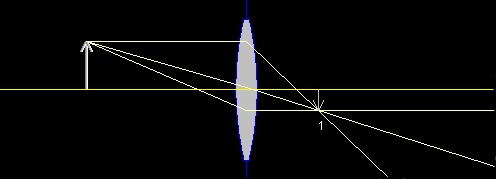
\includegraphics[scale=.7]{texlens1.png}
\end{center}
\end{figure}

\par
Também pode ocorrer que os raios aumentem a sua abertura. Neste caso, o ponto focal continua a existir, não como a intercepção dos raios mas antes como intercepção do prolongamento linear dos raios. Trata-se do caso das lentes divergente, ilustradas na Figura 2.


\begin{figure}[h]
\caption{Lente Divergente}
\begin{center}
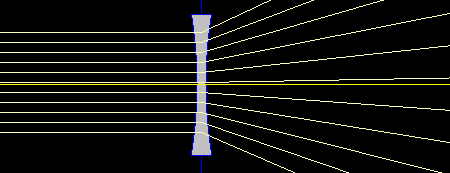
\includegraphics[scale=.7]{texlens2.png}
\end{center}
\end{figure}

\par 
Quando os raios provém de um objecto mais próximo, o ponto onde os raios convergem, também designado de imagem, não se encontrará na distância focal mas a uma distância {\it q}, dada pela seguinte equação, em função da distância focal {\it f} e a distância ao objecto {\it p}.

\begin{equation}
\frac{1}{f}=\frac{1}{p}+\frac{1}{q}
\end{equation}

\par
Esta equação é chamada a equação dos focos conjugados e o sinal das distâncias é dada conforme o objecto ou imagem sejam reais ou virtuais, sendo o sinal positivo ou negativo respectivamente. Entende-se por objecto ou imagem real aqueles onde os raios se interceptam, e por virtuais aqueles onde apenas o prolongamento linear dos raios se interceptam. Assim, a distância focal de uma lente convergente é sempre positiva, enquanto a distância focal de uma lente divergente é sempre negativa.

\subsection{Óptica da Luneta Terrestre}\index{Óptica da Luneta Terrestre}

A Luneta Terrestre é uma combinação bastante simples de uma lente convergente e uma lente divergente, em que a objectiva, a lente convergente, tem maior distância focal que a ocular, a lente divergente, estando a ocular colocada a uma distância da objectiva igual à diferença entre as distâncias focais.
\par
Esta combinação é utilizada para ampliar objectos a uma distância tal que possa ser tida como infinita. Quando a distância entre as lentes é exactamente igual à diferença entre distâncias focais, a imagem resultante é igualmente no infinito e não invertida, sendo a ampliação uma ampliação angular. Todavia, neste programa, para a imagem ser melhor visualizada, uma luneta é tomada com uma distância entre lentes próxima da diferença entre as distâncias focais, resultando numa imagem ampliada a uma distância finita.
\par
A luneta é assim bastante distinta do telescópio refractivo, ou telescópio kepleriano. Este utiliza duas lentes convergentes e a imagem resultante é invertida. Contudo, permite maiores ampliações, produz uma imagem melhor focada e tem um maior campo de observação.
 
\pagebreak
 
\section{Introdução à Utilização do Programa}
\index{Introdução à Utilização do Programa}

\subsection{Compilar o Programa}
\index{Compilar o Programa}
O programa "Galileo" é actualmente distribuido numa pasta com os ficheiros de texto com o código e uma Makefile. Para poder correr o programa após obtenção desta pasta deve fazer {\bf make} através da linha de comandos na pasta do programa. Caso ocorra alguma problema ou caso seja necessário eleminar os ficheiros .o e o ficheiro executável, pode inserir {\bf make clean} na linha de comandos na pasta em questão para apagar todos os ficheiros criados pela Makefile.
\par
Uma vez tendo compilado o programa, o executável é designado por {\bf galileo} e pode ser executado na linha de comandos através de {\bf ./galileo} na pasta em questão.

\subsection{Utilizar o Programa: Os Básicos}
\index{Utilizar o Programa: Os Básicos}
O objectivo do programa é permitir ao utilizador simular um sistema óptico que pode formar uma luneta mas que também pode ser manipulado para combinações ópticas com outros resultados, se bem que não é garantido que todos sejam produtivos. Como tal, o utilizador disponibiliza ao utilizar uma lente convergente, uma lente divergente e as ferramentas ao utilizador para as alterar.
\subsubsection{Posição das Lentes}
\index{Posição das Lentes}
O programa permite ao utilizador alterar a posição das lentes de duas formas distintas: através do rato ou através das barras horizontais no primeiro separador.
\par
Para alterar a posição das lentes do rato basta premir uma das lentes com o rato. Para premir uma lente basta premir qualquer ponto no rectângulo limitado pela altura e largura máxima da lente. Caso as duas lentes estejam sobrepostas, o programa dará prioridade à lente convergente. Uma vez estando a lente premida, basta deslocar o rato de forma a arrastar a lente ao longo do eixo óptico. A posição vertical das lentes não pode ser alterada. O programa também não permite que a lente seja posicionada fora dos limites da área de desenho.
\par
Para alterar a posição das lentes com as barras de ajuste basta seleccionar o separador {\bf Posição das Lentes} e alterar a posição de cada lente na barra respectiva.
\par 
A posição das lentes é dada em valor na caixa {\bf Dados} ou junto às barras. Este valor reflecte a posição na área de desenho em pixeis quando na escala {\bf 1:1}. Caso a escala esteja alterada deve ter em conta esse factor (para mais sobre escalas ver !!!!!!).

\subsubsection{Distância Focal das Lentes}
\index{Distância Focal das Lentes}

A distância focal de cada lente pode ser alterada de forma semelhante. No separador {\bf Distâncias Focais} existe uma barra de ajuste para cada distâncial focal, permitindo valores até 300.
\par
A distância focal também pode ser alterada com o rato. Junto a cada lente existe um círculo, laranja para a lente convergente e azul para a lente divergente, que representa a distância focal. Este círculo pode ser arrastado com o rato, aproximando-o o afastando-o da lente. A distância deste ponto à lente é a distância focal. Assim, aproximando este ponto da lente diminui a distância focal e afastando aumenta.
\par 
As distâncias focais das lentes também podem ser lidas na caixa {\bf Dados}.

\subsubsection{Ângulo de Incidência}
\index{Ângulo de Incidência}
Como o objecto observado pela luneta terrestre está muito distante, os raios provenientes são paralelos. Como tal, o parâmetro relevante sobre os raios que são recebidos pela luneta é o ângulo de incidência. Para alterar o ângulo de incidência basta utilizar a primeira barra de ajuste no separador {\bf Angulo/Escala}.

\pagebreak

\section{Outras Opções do Programa}
\index{Outras Opções do Programa}

\subsection{Escala}
\index{Escala}

No separador {\bf Angulo/Escala} é possível alterar a escala na segunda barra de ajuste. Alterar a escala reflecte uma multiplicação de todas as distâncias por um factor, ou seja funciona de forma semelhante a um zoom.
\par

\subsection{Raios Virtuais}
\index{Raios Virtuais}

Na caixa {\bf Opções} está disponível a opção {\bf Ver Raios Virtuais}. Entende-se por raios virtuais todas as linhas que reflectem prolongamentos de raios luminosos, sendo portanto caminho que não são percorridos por luz mas que têm valor físico e geométrico. Quando esta opção se encontra ligada, estes raios têm uma cor diferente e são desenhadas a tracejados. Quando desligadas, não são visíveis.
\par

\subsection{Fixar Distâncias}
\index{Fixar Distâncias}
Na caixa {\bf Opções} está disponível a opção {\bf Fixar Distâncias}. Enquanto esta opção estiver ligada a distância entre as lentes será conservada quando uma das lentes é alterada. Tal pode ser útil para deslocar um sistema óptico sem perturbar as suas características. Também limitará a alteração das lentes, de forma a que nunca seja possível arrastar uma lente para fora da área de desenho.
\par
\subsection{Recomeçar}
\index{Recomeçar}
O botão {\bf Recomeçar} altera as todas definições ajustáveis pelo utilizador aos valores iniciais. Isto inclui todas as barras de ajuste e butões.
\par
\subsection{Criar Luneta}
\index{Criar Luneta}
O botão {\bf Criar Luneta} altera as posições das lentes de forma a que formem uma luneta terrestre. Para tal, a distância focal da lente convergente deve ser maior que a distância focal. É recomendado que a diferença entre distâncias focais seja grande para que se veja bem a luneta.
\par
\subsection{Cores}
\index{Cores}
O botão {\bf Cores} abre um menu que permite ajustar as cores dos objectos desenhados. Isto  inclui as lentes (no modo "esquemáticas), os raios reais e virtuais e os objectos. Neste menu o botão {\bf Restaurar Cor} reverte a cor seleccionada para a cor predefinida e o botão {\bf Cores Predefinidas} restaura todas as cores.
\par
\par
\subsection{Bloqueado/Desbloqueado}
\index{Bloqueado/Desbloqueado}
O botão {\bf Bloqueado/Desbloqueado} é semelhante ao botão {\bf Criar Luneta}, excepto que enquanto estiver activo ("Bloqueado") o programa força a existência de uma luneta. Isto é, por um lado, a posição das lentes não pode ser alterada directamente, e, por outro, caso as distâncias focais sejam alteradas a posição das lentes é automaticamente ajustada para formar uma luneta.
\subsection{Tipo de Lentes} 
\index{Tipo de Lentes}
A caixa {\bf Tipo de Lentes} apresenta duas opções para o desenho das lentes. A opção {\bf Esquemáticas} desenha as lentes como rectas encabeçadas por triângulos, como é padrão em esquemas de sistemas ópticos. A opção {\bf Desenhadas} desenha de uma forma ilustrativa as lentes, com um perfil de lente esférica cujo raio varia com a distância focal de forma qualitativamente semelhante ao previsto pela teoria.

\par
\end{document}

-----------> footnotes
